\section{Actuation module}

After the \emph{perception} tasks, the system has obtained the maximum possible certainty about the persons present in the current RGB image, as well as their condition of being or not being the one to be followed.\\

The next functional block, the \emph{actuation} one, is responsible of generating a suitable command to the robot motors, in order to move towards the followed person, in case it is being seen in the current frame. To do so, it follows its own pipeline, explained next.


\subsection{Following behavioral}

As it has been stated, the input for this element is the information yielded by the \emph{perception} block: the \emph{tracked persons} parameters (position, face, ``is or not the followed person"). From this information, the new \emph{actuation} block has to infer which attitude to take (depending on the state of the system on the last iteration). This is implemented with a \emph{case-based} behavioral, which follows the \emph{flow chart} represented on Fig. \ref{fig:actuation_flow}. It can be seen that the response depends on \emph{mom} (the semantical name given to the followed person), as it can be \emph{lost} or \emph{tracked and followed}.\\

\begin{figure}[h]
	\centering
	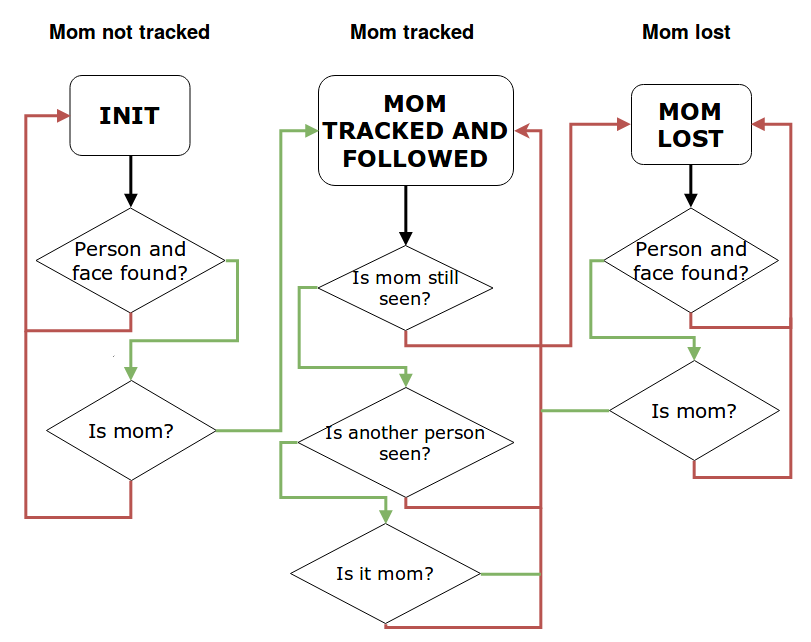
\includegraphics[width=2.5in]{images/flowchart}
	\caption{\emph{Flow chart} followed by the case-based behavioral, depending on the previous state.}
	\label{fig:actuation_flow}
\end{figure}

If the followed person is found among the tracked persons, the system follows it. It can observed as well that, as it was mentioned before, the system does not need a continuous face feedback to follow the target person, as it just needs to be still seen (that time-spatial continuity is provided by the previously described trackers). In addition, if a new face is found, and it satisfies the criteria of similarity with the reference face, the \emph{followed} role is swapped to that new person, which begins to be followed by the system.\\


\subsection{Error computation}

Once the system has recognized the target person into the image, in case it is being seen, it proceeds to an \emph{error computation}, in order to determine the strength of the required movement to move towards that person. As the robot used on the proposed system moves in two dimensions, we perform a dual error computation:

\begin{itemize}
	\item \emph{Angular error:} the most accurate position for the system with respect to the person is to be aligned with it. This way, the person appears right in the horizontal center of the image. Hence, we can compute the \emph{angular error} as the subtract of the center coordinates and the center of the person's bounding box, in the horizontal dimension. This process,  represented in Fig. \ref{fig:h_error}, will give a quantization of the necessary turn to be performed.\\
	
	\begin{figure}
		\centering
		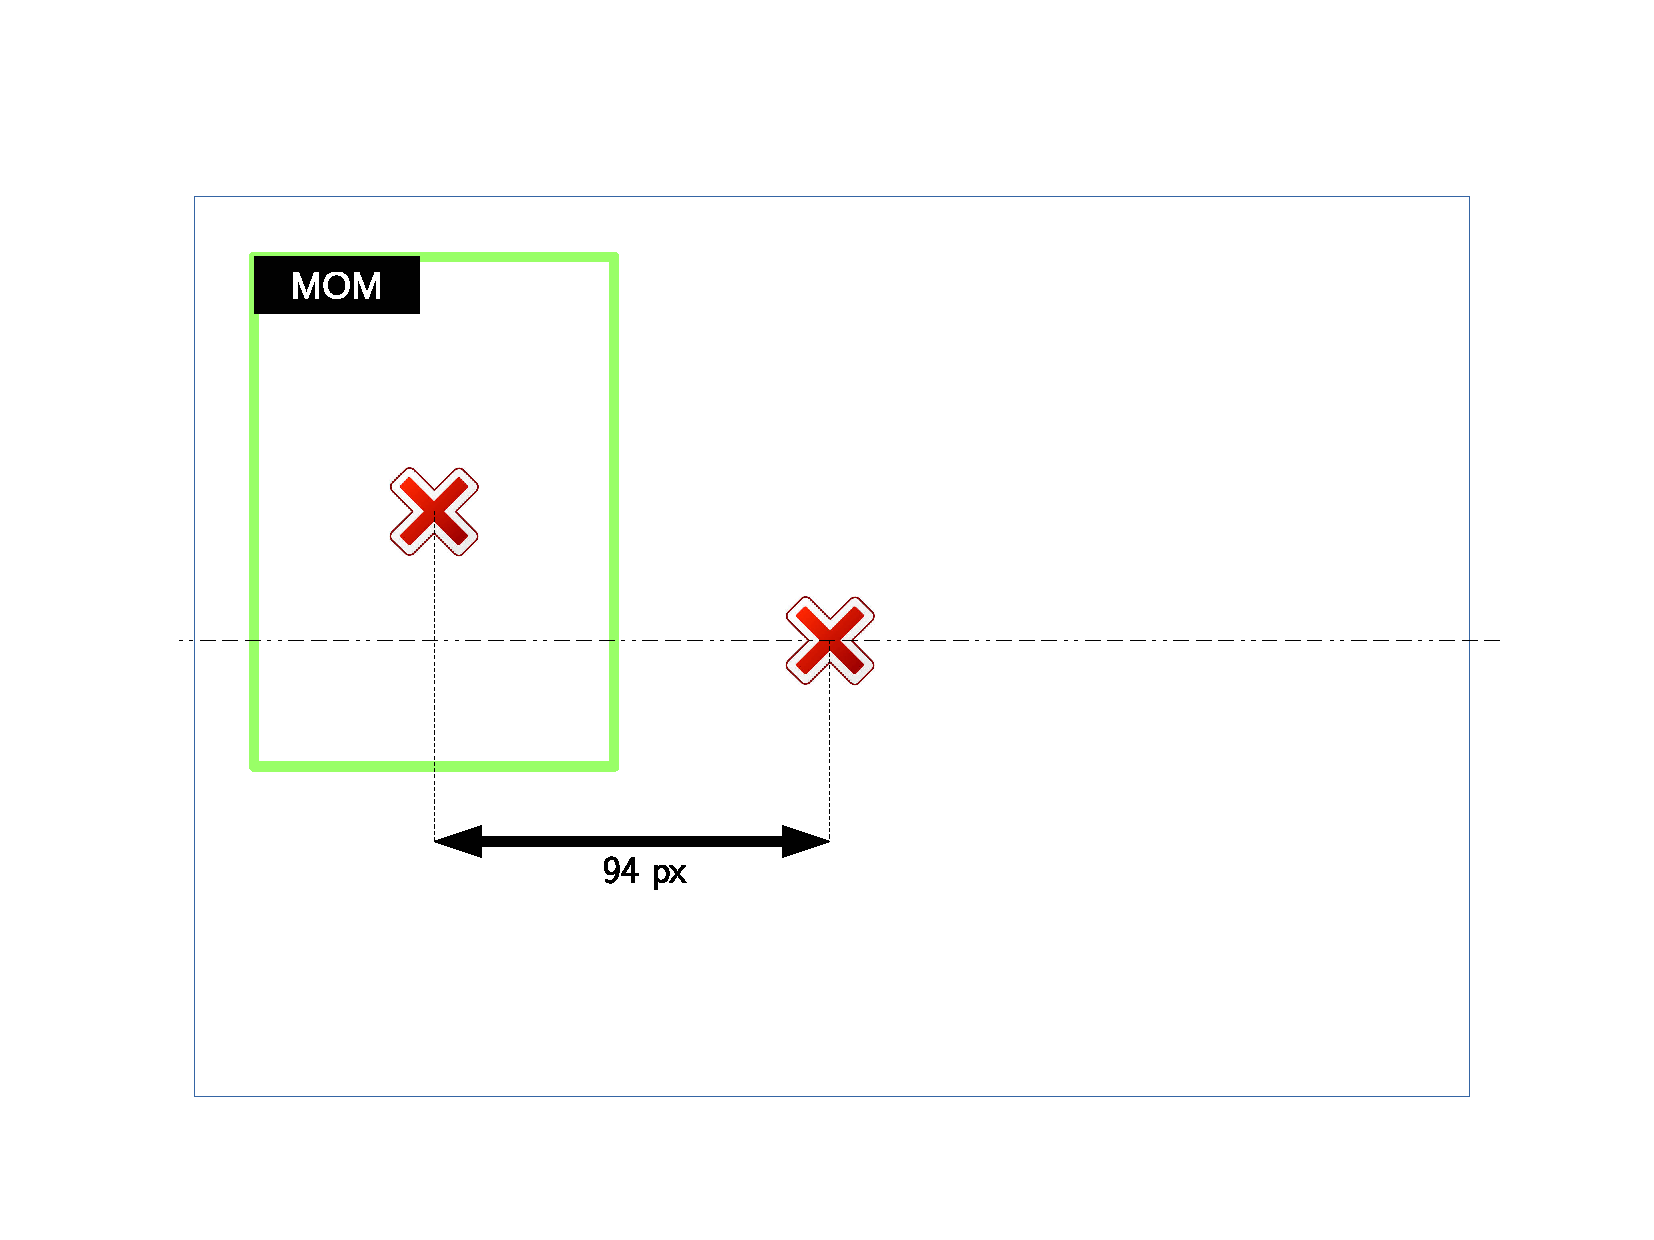
\includegraphics[width=2.4in]{images/h_error}
		\caption{Computation of the angular error between the system and the followed person.}
		\label{fig:h_error}
	\end{figure}
	
	
	\item \emph{Linear error}: as the implemented sensor is a RGBD camera, it will provide the system a \emph{depth} image. As it is aligned with the RGB image, the coordinates of the person inside the depth image are the same than the RGB ones. Hence, it allows to \emph{locate} the person inside the depth map.\\
	
	In consequence, a 10$\times$10 grid sampling of the depth values inside the person box (putting care on avoiding the margins, in order to measure only inside the person) allows to collect a serie of measured distances to the person. This system performs that process, and computes the \emph{median} of that set of measures, taking the result as the distance from the robot to the person, as seen on Fig. \ref{fig:v_error}.
	
	
	\begin{figure}[h]
		\centering
		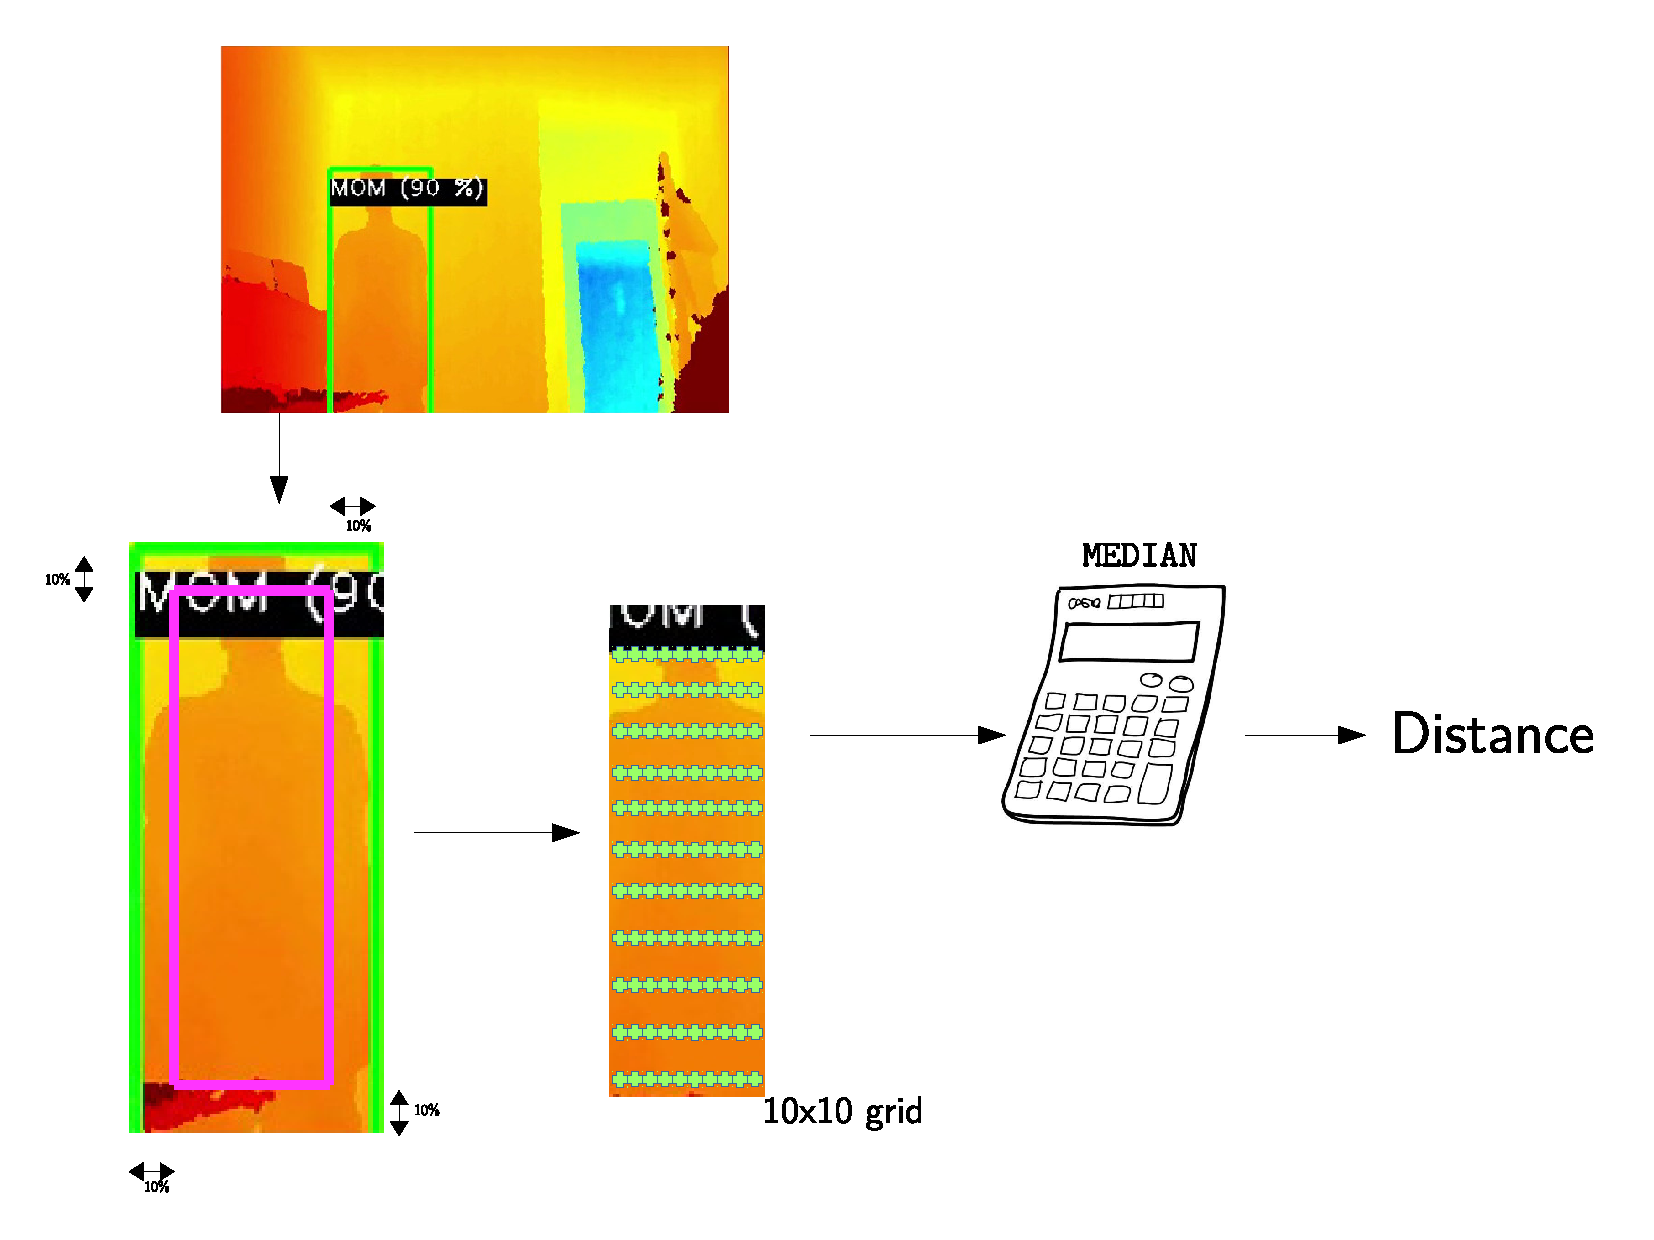
\includegraphics[width=2.5in]{images/distance_error}
		\caption{Computation of the linear error between the system and the followed person.}
		\label{fig:v_error}
	\end{figure}
	
\end{itemize}


So far, the system is capable to determine a numerical error value to measure the magnitude of the required response.\\


\subsection{Movement response}

The previous measures are required to determine the \emph{relative position} of the robot and the target person. It is used as an input to compute the most suitable response.\\

As the system is not designed to move literally to the position of the person, but to just maintain a following behavior, a \emph{dead zone} is established in each dimension. These dead zones (illustrated on Fig. ) will cause the robot not to move anymore towards the person, as the person is considered \emph{under control} when it is placed inside.\\


\begin{figure}[h]
	\centering
	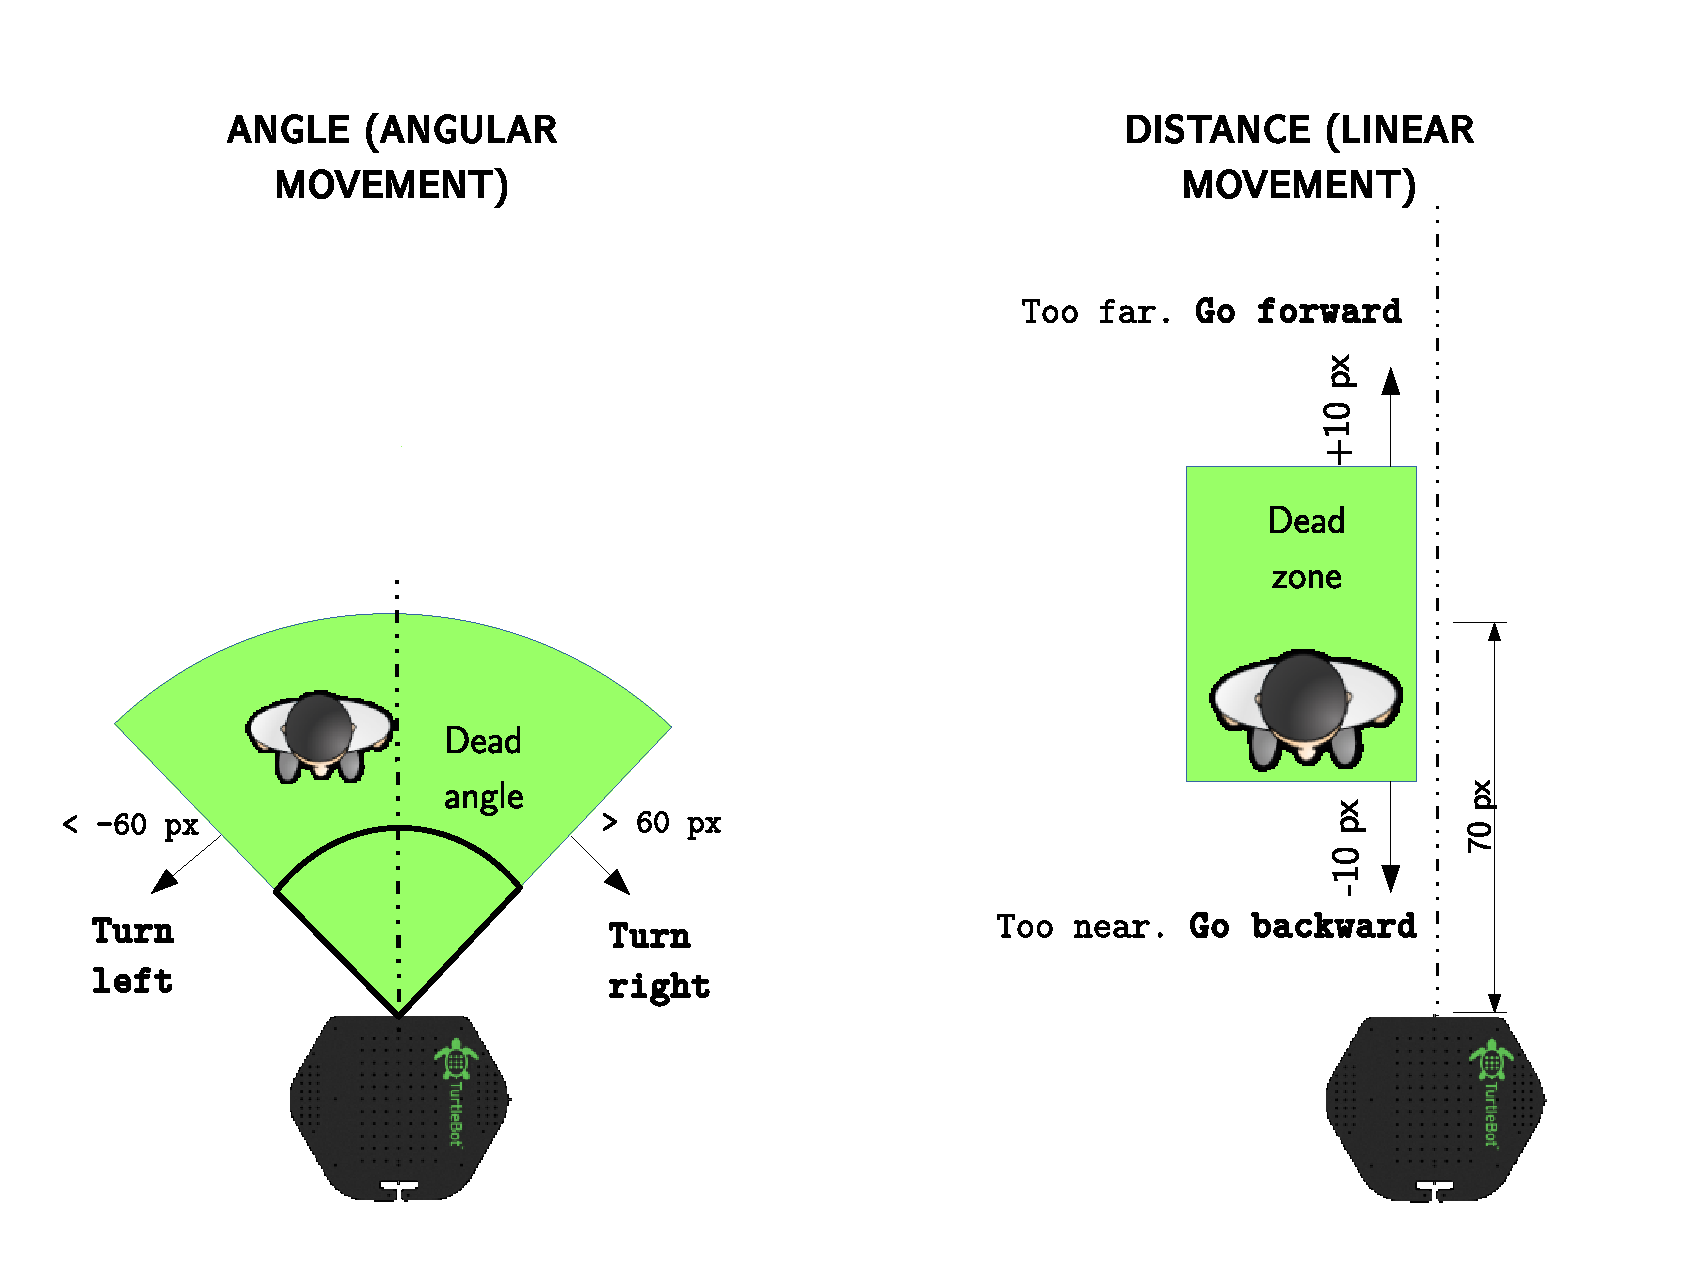
\includegraphics[width=2.5in]{images/dead_zones}
	\caption{Dead zones on each dimension, where the person is considered under control.}
	\label{fig:dead_zones}
\end{figure}


If the person is outside these dead zones, a physical response is required, with the purpose of \emph{carrying} that person inside the dead zone. For this action, each dimension implements a \emph{PID} controller, which establishes a \emph{closed-loop} feedback system, as described on \cite{pid-controller}. This allows to keep in mind previous responses, to achieve the optimum fitting in every iteration. This means, for example, to accelerate if the person is not going any closer, or to step hard on the brake if the person suddenly gets too close.\\

The implemented \emph{PID} controllers (an angular and a linear one) have been experimentally tuned to obtain the most suitable parameters for our operation, obtaining the values in Table \ref{tab:pids}.\\

\begin{table}[h]
	\centering
	\begin{tabular}{|c|c|c|}
		\hline
		\textbf{} & \textbf{Linear} & \textbf{Angular} \\ \hline
		$k_p$     & 2               & 7                \\ \hline
		$k_d$     & 0.1             & 0.5              \\ \hline
		$k_i$     & 3               & 10               \\ \hline
	\end{tabular}
	\caption{Optimal found values for the parameters in each PID controller.}
	\label{tab:pids}
\end{table}

This way, the system can output a speed value with a tight adjustment to the values required by the situation of the current iteration. The response obtained from this value is a \emph{reactive} one. This means that each value results in a new movement command, avoiding to perform movements longer than one iteration. For softness sake, what is sent to the motors is not this value, but the \emph{mean} between it and the last sent one. This way, it results on a slightly longer convergence that helps to remove sudden movements.





\vspace{1.5in}

The previously described pipeline is executed \emph{once} per thread iteration, maintaining on concurrent threads each one of the two blocks (\emph{perceptive} one and \emph{actuative} one). This results on a new speed command to each one of the two available motors (angular and linear advances) on each iteration.